\documentclass{article} % For LaTeX2e
\usepackage{nips14submit_e,times}
\usepackage{hyperref}
\usepackage{url}
\usepackage{graphicx}
\usepackage{subcaption}
%\documentstyle[nips14submit_09,times,art10]{article} % For LaTeX 2.09


\title{An Analysis of the Web Graph Utilizing Apache Flink}
\author{
Hung Chang \\
\and
Philip Raschke
}

% The \author macro works with any number of authors. There are two commands
% used to separate the names and addresses of multiple authors: \And and \AND.
%
% Using \And between authors leaves it to \LaTeX{} to determine where to break
% the lines. Using \AND forces a linebreak at that point. So, if \LaTeX{}
% puts 3 of 4 authors names on the first line, and the last on the second
% line, try using \AND instead of \And before the third author name.

\newcommand{\fix}{\marginpar{FIX}}
\newcommand{\new}{\marginpar{NEW}}

%\nipsfinalcopy % Uncomment for camera-ready version

\begin{document}

\maketitle

\begin{abstract}
This project aims to achieve a comprehensive analysis of the structure of the World-Wide-Web. Therefore, we used the data sets provided by the Web Data Commons project which extracted the web graph from the Common Crawl project. A small example data set was used while implementing algorithms that compute degree, connectivity, PageRank, closeness and betweenness of the nodes of the graph. Graph analyzing tools were used to evaluate the algorithms' validity. The computations then were run on a four node cluster on larger data sets to retrieve results of the whole web graph.
\end{abstract}

\section{Problem Statement}
In the last years a vast amount of data has been collected and has been made available to the public in order for everyone to analyze this data and gain knowledge about its structure. One example for such data set is the Hyperlink Graph of the University of Mannheim which has been extracted from the Common Crawl. There are currently two versions of the graph namely the 2012 and 2014 version each covering billions of pages and hyperlinks between those pages. Analyzing this data set may be beneficially for multiple research fields like  search algorithms, SPAM detection or graph analysis algorithms.  
 
The target of this project is to implement algorithms to compute the statistics of importance such as indegree and outdegree distribution, the PageRank, the closeness and the betweenness centrality. Those statistics rank the nodes from different aspects. A major challenge within the implementation part is the scalability of the algorithms. Since the data set consists of millions of nodes, it is strictly required to efficiently compute the different measures. Especially the closeness and betweenness centrality are resource intensive computations. Therefore, those algorithms will be implemented according to Kang et al. [1].

Further, another goal is to analyze the data set with the help of Apache Flink to process huge parts of the data set. Based on the results statements can be made about the structure of the Hyperlink Graph and therefore statements can be formulated about the structure of the World-Wide-Web. Based on the results retrieved from the computations, comparisons will be made to results of other research. Various research groups already analyzed the structure of the web graph [4]. These results can be confirmed or rejected by results retrieved from this project.

\section{Methodology}
Centrality is a measure which indicates the importance of a node. The degree of a node is the most common and basic measure in the field of network analysis. The degree centrality counts the number of paths of length 1 that emanate from a node. Another degree centrality measure instead is the PageRank, which simulates a random walk on the graph. The rank gives the probability a surfer reaches the respective page. 

The second group of centrality measures is the group of diameter related measures, which count the length between nodes. The closeness for example takes the diameter into account in order to identify a nodes’ importance. A general definition of closeness is based on the length of the average shortest path between a node and all other nodes in the network. 

The third measure is the betweenness which considers the flow. A general definition of the betweenness is the number of node pairs that need to go through a node in order to reach each other taking the minimum number of hops. Figure \ref{fig1} shows the three groups of measures.

\begin{figure}[H]
	\begin{center}
		\label{fig1}		
		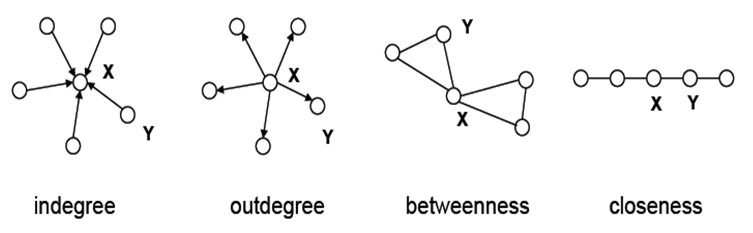
\includegraphics[width=0.6\textwidth]{fig1}	
		\caption{Measures overview}	
	\end{center}
\end{figure}

\subsection{Degree, indegree and outdegree}
The degree is a fundamental measure within the analysis of networks. It gives some indication of a nodes position in the network. The indegree of a vertex in a directed graph is given by the number of edges pointing to the respective vertex. The outdegree on the contrary gives the number of edges coming from the corresponding node. In order to efficiently compute the both degrees, we build the adjacency matrix of the network and count the neighbors of node with MapReduce. Besides, we also write a top K degree computation to focus on higher degree node.

\subsection{Degree distribution}
The degree distribution is the probability distribution of the degrees over the whole network. This project scalable computes them by using the MapReduce model using the degree as key in a key-value pair. The subsequent reduce job builds the sum of these key-value pairs and so builds the degree distribution.

\subsection{PageRank}
The PageRank algorithm was developed by Google founders Larry Page and Sergej Brin at Stanford University in 1996. The algorithm is used to rank pages in order to measure the importance of websites. Therefore, the algorithm computes a probability distribution representing the likelihood that a user reaches a specific web page by randomly clicking on links. In order to compute the PageRank, we run the algorithm in iterations. To handle circles in the graph, which might prevent the algorithm from converging, we implemented the random teleport behaviour. Nodes without outgoing edges have been modified in a way that these point to all other nodes in the network visualized as green arcs in Figure \ref{fig2}. We also want to focus on higher PageRank and write a top K PageRank.

\begin{figure}[H]
	\begin{center}
		\label{fig2}		
		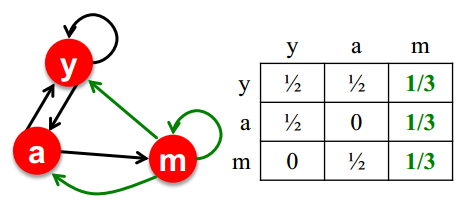
\includegraphics[width=0.6\textwidth]{fig2}	
		\caption{PageRank sinks}	
	\end{center}
\end{figure}

\subsection{Closeness centrality}
Closeness measures the importance of a node based on the distance to other nodes in the network. The intuition of the large-scale algorithm is to count approximately the number of neighbors that a node connects to at each step of the iterative computation. This approach is proposed by Kang et al. in their paper “Centralities in Large Networks: Algorithms and Observations” [1]. Effective Closeness is a large-scale centrality algorithm. 

Following Figure \ref{fig3} shows a toy example showing the intuition. For node 1, at step 1, it connects to two nodes, at step 2, it connects to two nodes and at the final step, it  connects one node. Therefore, node 1’s count is given by 1 * 2 + 2 * 2 + 3 * 1 = 9. For node 3, the count is 3 * 1 + 2 * 2 = 7. It is observable that node 3 is more central than node 1. The closeness supports this since node 3’s count is less than node 1’s count. Note that the closeness does not consider the direction of edges.

\begin{figure}[H]
	\begin{center}
		\label{fig3}		
		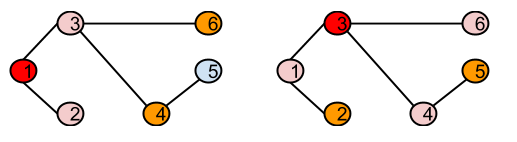
\includegraphics[width=0.6\textwidth]{fig3}	
		\caption{Closeness}	
	\end{center}
\end{figure}

The other scalable skill applied is the count distinct elements skill in data stream which is called Flajolet-Martin (FM).  When observing a stream of random integers, see an integer which binary representation starts with limited buckets, there is a higher chance that the cardinality of the stream is 2\^\ (size of the limited buckets). For instance, 25\% of bits start with "01", 12,5\% starts with "001" and if the limited bucket show "001", the estimated cardinality is 8. Thus, effective closeness algorithm uses bitstring to represent nodes and update the next step with bitwise OR. 

+Originally, the algorithm is designed for undirected graphs, thus, this project firstly transforms the directed Hyperlink Graph into an undirected graph, and then applies the described algorithm on it. We want to focus on higher closeness nodes rather than all nodes, thus, our program runs as a top K closeness

\begin{figure}[H]
	\begin{center}
		\label{fig4}		
		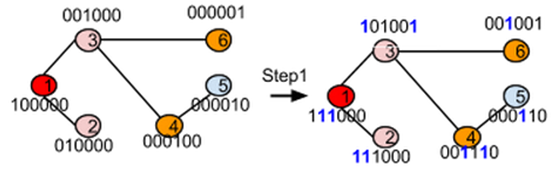
\includegraphics[width=0.6\textwidth]{fig4}	
		\caption{One step of closeness computation}	
	\end{center}
\end{figure}

\subsection{Betweenness centrality}
The betweenness centrality of a node in a network is given by the number of shortest paths from any other node to another node that passes the respective node. It is therefore an indicator of a nodes’ importance or centrality. To calculate it, the intuition is to score each edge by “power iteration” and then calculate the importance of nodes by aggregating the edges’ score. This approach is as well proposed by Kang et al. in the paper “Centralities in Large Networks: Algorithms and Observations”. For the Hyperlink Graph in this project, the implementation pre-processes the graph by removing dead-ends and transform the directed graph into undirected graph.

\begin{figure}[H]
	\begin{center}
		\label{fig5}		
		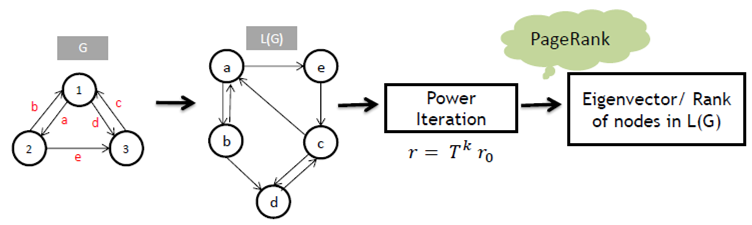
\includegraphics[width=1.0\textwidth]{fig5}	
		\caption{Betweenness}	
	\end{center}
\end{figure}

The intuition of the betweenness, which is also called LinkRank, is that some edges are important since many nodes have to go through them to reach other nodes. This flow-based measure is similar to the main road and branch approach. Nodes that connect to the main roads are more important. Thus, the scalable calculation of the betweenness uses similar measures to the PageRank way in order to identify more important edges in the network.

Based on the description above, the first step is to transform the graph G into a line graph L(G) where nodes become arcs and edges become nodes, respectively. The scalable idea here is instead of materializing L(G), decomposing L(G) by S(G) x T(G) which are in-edges and out-edges. 

\begin{figure}[H]
	\begin{center}
		\label{fig6}		
		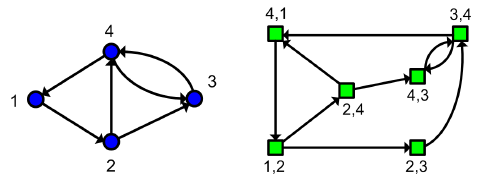
\includegraphics[width=0.8\textwidth]{fig6}	
		\caption{Graph G and its line graph L(G)}	
	\end{center}
\end{figure}

\begin{table}[t]
	\caption{S(G) and T(G)}
	\label{t1}
	\begin{center}
		\begin{tabular}{|l|l|l|l|l|l|}
			\hline
			S(G)	&	&	&T(G)	&	&	\\ \hline
				&source	&	&	&target	&	\\	\hline
			arc1	&1	&1	&arc1	&2	&1	\\ \hline
			arc2	&2	&1	&arc2	&3	&1	\\ \hline
			arc3	&2	&1	&arc3	&4	&1	\\ \hline
			arc4	&3	&1	&arc4	&4	&1	\\ \hline
			arc5	&4	&1	&arc5	&1	&1	\\ \hline
		\end{tabular}
	\end{center}
\end{table}

The next step in the computation is the calculation of the eigenvector S(G) multiplied by T(G) which is the same as the PageRank which is given by the stationary probability. After finishing the computation of the arcs importance score, the scores are summed up to retrieve the final LineRank score for each node T.


\section{Experiments}
\subsection{Apache Flink}
Apache Flink is a large-scale data processing engine optimal to process large amounts of data. It offers APIs for Java, Scala and hadoop MapReduce as well as various APIs to access data. Flink programs can be run locally on a single machine or on a cluster of multiple nodes. When ran on cluster, load distribution and fault tolerance are handled by Apache Flink independently with few configuration effort. Flink enables processing huge amount of data while offering an easy to use API for programmers to implement algorithms.

\subsection{Web Data Commons}
The Web Data Commons is project of the University of Mannheim which is supported by the European Union, Amazon Web Services in Education Grant Award and by the German Research Foundation (DFG). The project offers data sets of the web graph to the public. The data sets were extracted from the Common Crawl Foundation which provides a web corpus to the public.

\subsection{Data sets}
There are multiple data sets offered by the Web Data Commons project differed by year and aggregation level. They offer the Hyperlink Graph 2012 and Hyperlink Graph 2014. Due to different crawling strategies which were used to gather the web corpora, the authors suggest to use the Hyperlink Graph 2012 for comprehensive network analysis of the web graph.

For the Hyperlink Graph 2012 there are the following four different aggregation levels. Page Graph, Subdomain/Host Graph, 1st Subdomain Graph and Pay-Level Domain Graph (PLD).

The Page-Level Graph represents every web page with all details as single node in the graph. An example for a node in this graph would be: dima.tu-berlin.de/menue/database\_ systems\_ and\_ information\_ management\_ group/

The Host Graph aggregates the Page Graph by the subdomains and hosts. Therefore, each subdomain is represented as node within the Host Graph. The two pages tu-berlin.de and dima.tu-berlin.de are two different nodes within this graph.

The PLD reduces the Host Graph by merging the subdomains with their host. The two nodes tu-berlin.de and dima.tu-berlin.de are represented in the PLD as a single node tu-berlin.de.

It is obvious that the size of the graphs decreases with the increase of the granularity level. The graphs are separated into two different files, namely an index file and an arc file. The index file consists of tuples which hold an identifier and the node name. The arc file gives tuples of two identifiers representing a link from one node to another. An overview of the different sizes is given by the following table.

\begin{table}[H]
	\caption{Number of Nodes and Arcs}
	\label{t2}
	\begin{center}
		\begin{tabular}{|l|l|l|}
			\hline
			Data Set	&\#Nodes	&\#Arcs \\ \hline
			Page Graph	&1,727M	&64,422M	\\	\hline
			Subdomain/ Host Graph	&22M	&123M	\\	\hline		
			PLD Graph	&13M	&56M	\\	\hline				
		\end{tabular}
	\end{center}
\end{table}

\subsection{Computation}
We initially planned to run the computations of the algorithms on a ten node cluster. Therefore, we initially intended to use the Host Graph as data set to achieve a comprehensive  analysis of the web graph. Unfortunately, due to organizational problems we were not able to run the computation on the cluster.

As a fallback plan, we decided to run the computation locally on our machines. Very first steps however, revealed that computing these amount of data on a single machine is not feasible, since our machines do not have enough memory. Hence, we reduced the data set to the PLD. This reduction allowed us to compute the indegree distribution and the Top-K outdegree of the PLD. These results were achieved on a machine with 3GB RAM and 2 processors with 2 cores. The computation took around 40 minutes. 

Other implemented algorithms such as the PageRank, closeness and betweenness could not be executed since our machines ran out of memory during the computation.

During the course of the project we were able to run the algorithms on a four node cluster. A detailed view on the configuration of the four node cluster can be seen in Figure \ref{fig6a}. This time we used the Host Graph as well as the PLD Graph as fallback. The computation of the indegree and outdegree was successful on the four node cluster. For both graph levels we were able to retrieve results. Nevertheless, the other algorithms to measure the connectivity, PageRank and closeness of the graph faced memory issues on the four node cluster.

\begin{figure}[H]
	\begin{center}
		\label{fig6a}		
		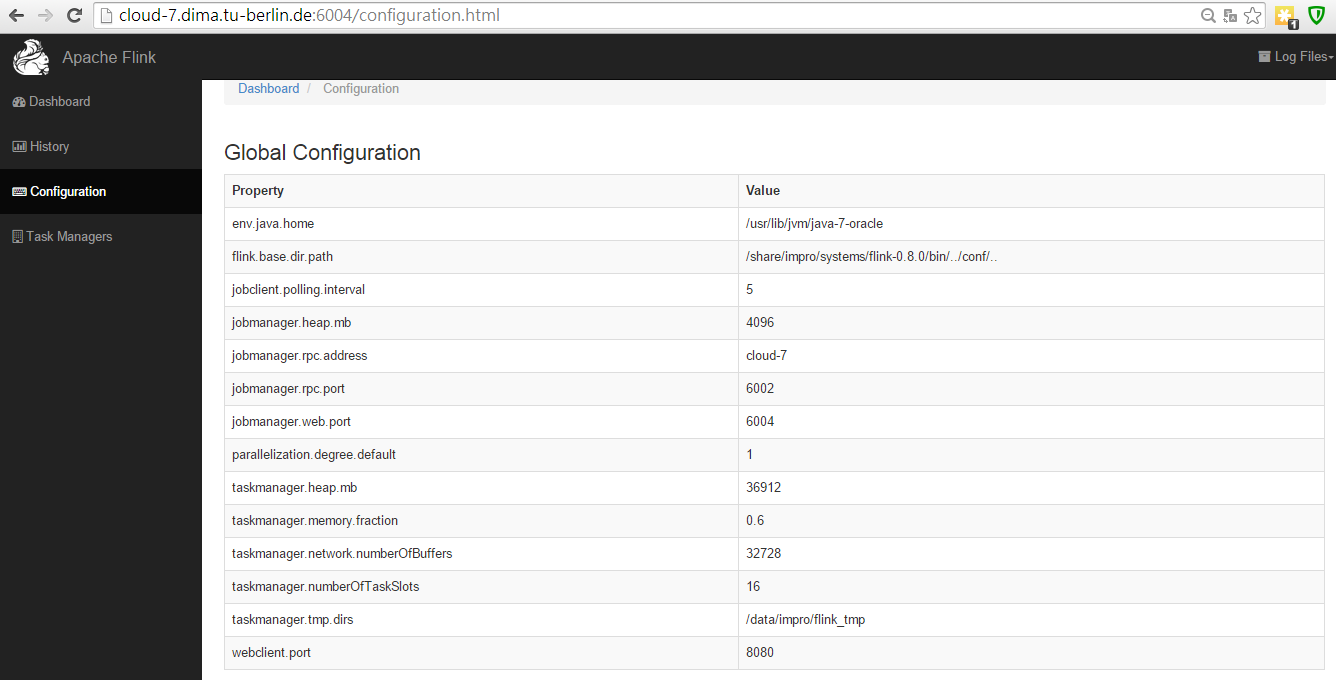
\includegraphics[width=1.0\textwidth]{fig6a}	
		\caption{Configuration of the 4-node cluster}	
	\end{center}
\end{figure}

\begin{table}[H]
	\caption{Computation overviews}
	\label{t3}
	\begin{center}
		\begin{tabular}{|l|l|l|l|}
			\hline		
				&Example graph (locally)	&PLD graph	&Subdomain-Host graph \\ \hline
			Degree	&Correct	&Correct	&Correct \\ \hline
			Connectivity	&Correct	&Memory issue	&Memory issue	\\ \hline
			PageRank	&Correct	&Memory issue	&Memory issue	\\ \hline
			Closeness	&Correct	&Memory issue	&Memory issue	\\ \hline
			Betweenness	&Correlation is 0	&Not run in cluster	&Not run in cluster	\\ \hline
		\end{tabular}
	\end{center}
\end{table}

\subsection{Evaluation}
To rapidly test our implementations of the different algorithms we used an example data set provided by the Web Data Commons project. This data set contains 106 nodes and 141 arcs. The Web Data Commons project provides results for the indegree and outdegree (see Figure 7 and 8). A comparison to these results show that our implementation in respect to the indegree and outdegree is correct and computes the expected results.

\begin{figure}[H]
\begin{minipage}{.5\textwidth}
	\begin{center}
		\label{fig7}		
		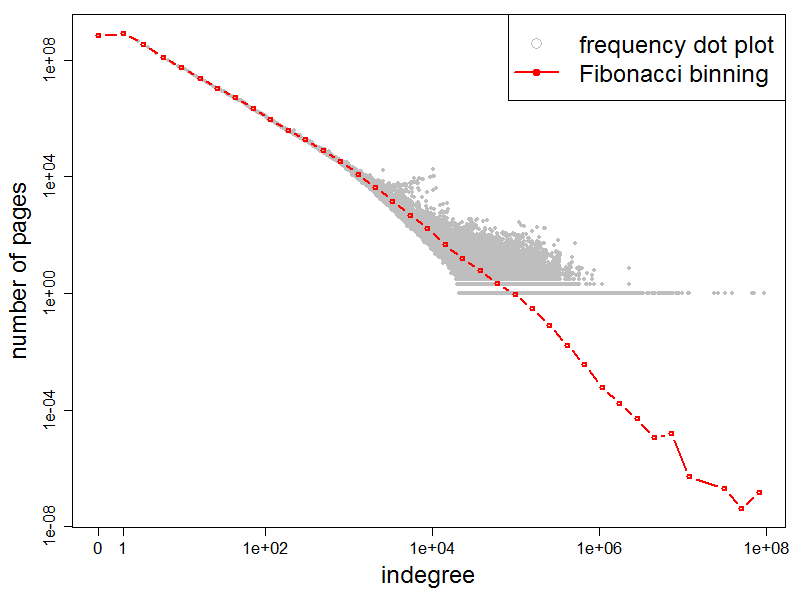
\includegraphics[width=1.0\textwidth]{fig7}	
		\caption{Indegree Distribution}	
	\end{center}
\end{minipage}
\begin{minipage}{.5\textwidth}
	\begin{center}
		\label{fig8}		
		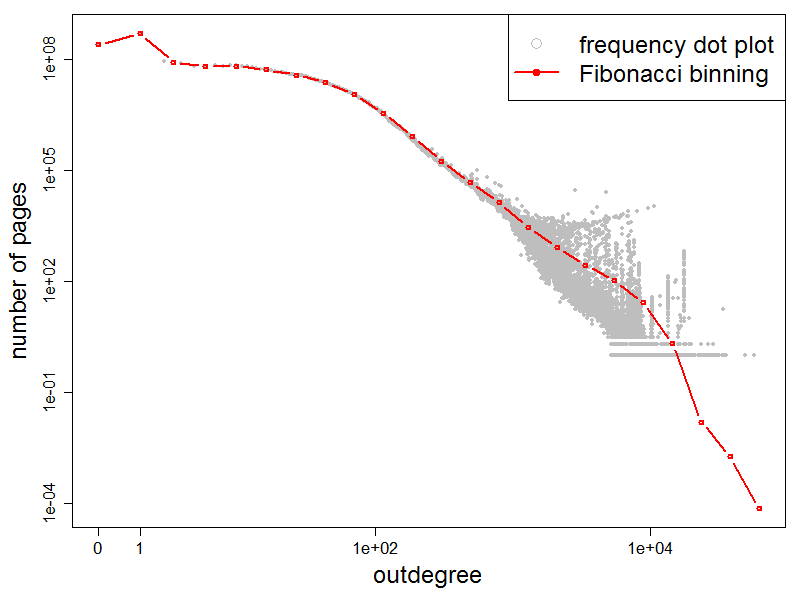
\includegraphics[width=1.0\textwidth]{fig8}	
		\caption{Outdegree Distribution}	
	\end{center}
\end{minipage}
\end{figure}

Further, we used the graph visualization tool Gephi which also provides computation functionalities for the measures degree, PageRank and closeness of graph. We compared our results to the results of Gephi and computed the Pearson correlation between the two result sets.
The correlation coefficient of the two different PageRank results is 1 (see Figure \ref{fig9}). The correlation coefficient for the Closeness results is 0.985 (see Figure \ref{fig10}). This shows that our implementation of the algorithms computes correct results.

\begin{figure}[H]
\begin{minipage}{.5\textwidth}
	\begin{center}
		\label{fig9}		
		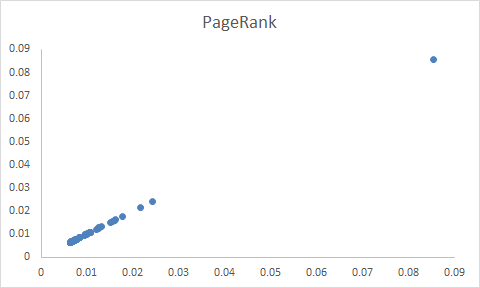
\includegraphics[width=1.0\textwidth]{fig9}	
		\caption{Correlation our results Gephi’s results (PageRank)}	
	\end{center}
\end{minipage} %
\begin{minipage}{.5\textwidth}
	\begin{center}
		\label{fig10}		
		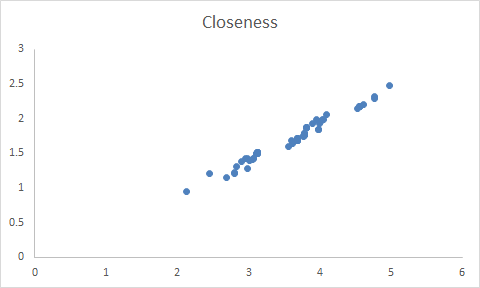
\includegraphics[width=1.0\textwidth]{fig10}	
		\caption{Correlation our results Gephi’s results (Closeness)}	
	\end{center}
\end{minipage}
\end{figure}

\section{Results}
The results of our computation are very limited due to the lack of computation power. We retrieved results from the computation of the indegree and outdegree which can be seen in Figure \ref{fig12} and Figure \ref{fig13}. Since these are our only results, we try to gain as much information from it as we can. Nevertheless, the results of our indegree distribution show the power-law. Yet, tt is observable that the, whether indegree distribution nor the outdegree distribution do not follow a strict linear regression, therefore, we applied  a regression ANOVA to confirm or reject the significance of a power-law.

\begin{figure}[H]
\begin{minipage}{.5\textwidth}
	\begin{center}
		\label{fig12}		
		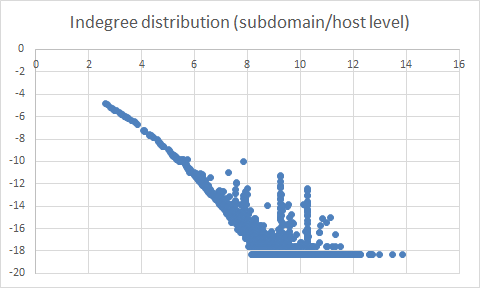
\includegraphics[width=1.0\textwidth]{fig12}	
		\caption{Indegree distribution}	
	\end{center}
\end{minipage} %
\begin{minipage}{.5\textwidth}
	\begin{center}
		\label{fig13}		
		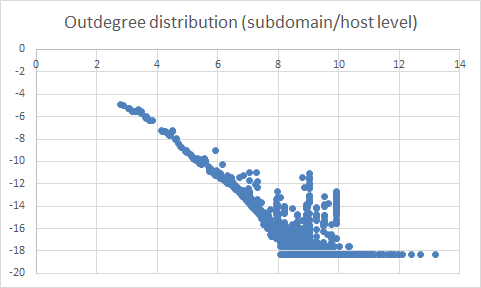
\includegraphics[width=1.0\textwidth]{fig13}	
		\caption{Outdegree distribution}	
	\end{center}
\end{minipage}
\end{figure}

The regression ANOVA (see Figure \ref{fig14}) reveals that the p-value is significant which is 0. However, one of the residual plots, which is the relationship between fitted value (predicted value) and residual, indicates the line is not a regression line (see Figure \ref{fig15}). The reason there is that the residuals have patterns, which violates the assumption of regression that the residuals must have no patterns. Besides, the data also does not follow the assumption that should be normal distribution based on the probability graph. In conclusion, the power-law is not significant. We can therefore confirm the results of other research [4].

\begin{figure}[H]
\begin{minipage}{.5\textwidth}
	\begin{center}
		\label{fig14}		
		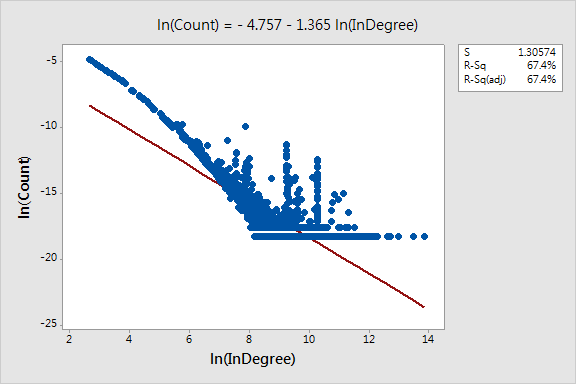
\includegraphics[width=1.0\textwidth]{fig14}	
		\caption{Regression ANOVA}	
	\end{center}
\end{minipage} %
\begin{minipage}{.5\textwidth}
	\begin{center}
		\label{fig15}		
		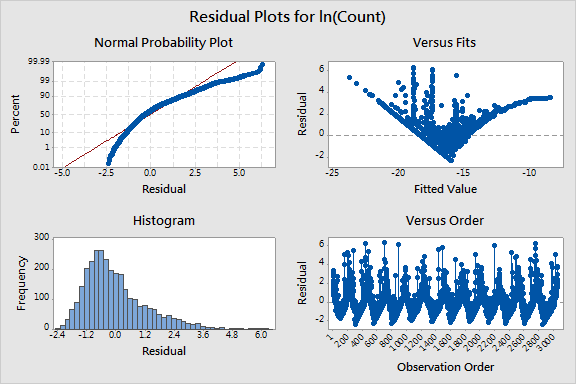
\includegraphics[width=1.0\textwidth]{fig15}	
		\caption{Residual Plots}	
	\end{center}
\end{minipage}
\end{figure}

The results of our Top-10 indegree computation can be seen in Table \ref{t4a}. Further, see Table \ref{t4} for the results of our Top-10 outdegree computation. These results are also confirmed by the Web Data Commons project \footnote{Topology of the 2012 WDC Hyperlink Graph. URL: http://webdatacommons.org/hyperlinkgraph/2012-08/topology.html\#toc9 Last accessed: 10th of February 2015}.

\begin{table}[H]
	\caption{Top-10 Indegree (Host Graph)}
	\label{t4a}
	\begin{center}
		\begin{tabular}{|l|l|}
			\hline
			Website	&Indegree \\ \hline
			wordpress.org	&2,335,856 \\ \hline
			youtube.com	&2,073,535 \\ \hline
			gmpg.org	&1,784,793 \\ \hline
			en.wikipedia.org	&1,545,864 \\ \hline
			twitter.com	&1,036,611 \\ \hline
			google.com	&798,348 \\ \hline
			rtalabel.org	&657,414 \\ \hline
			wordpress.com	&646,766 \\ \hline
			mp3shake.com	&549,122 \\ \hline
			w3schools.com	&507,184 \\ \hline
		\end{tabular}
	\end{center}
\end{table}

\begin{table}[H]
	\caption{Outdegree and Page views}
	\label{t4}
	\begin{center}
		\begin{tabular}{|l|l|l|}
			\hline
			Website	&Outdegree	&Page views \\ \hline
			serebella.com	&699609	&3 \\ \hline
			tumblr.com	&496045	&7.18 \\ \hline
			blogspot.com	&3898561	&3.21 \\ \hline
			wordpress.com	&2249553	&4.71 \\ \hline
			refertus.info	&668271	&1 \\ \hline
			typepad.com	&551360	&1.89 \\ \hline
			botw.org	&496645	&2.82 \\ \hline
			top20directory.com	&650884	&1.3 \\ \hline
			wikipedia.org	&862705	&3.53 \\ \hline	
			youtube.com	&1078938	&6.08 \\ \hline			
		\end{tabular}
	\end{center}
\end{table}

\section{Conclusion}
The goals of this project have been partly achieved. The implementation of the algorithms in order to compute the different measures have been fully completed. An evaluation of these algorithms showed that the implementations produce correct results, including degree, connectivity, PageRank, closeness, except that betweenness doesn't match Gephi's betweenness computation. For this evaluation an example data set was used to rapidly test the algorithms, and compare the results of our algorithms with Gephi's result. Due to lack of computation power, we first tried to run the computations locally, and reduced the granularity from the Subdomain/Host Graph to the PLD graph. Then, we use the 4-node cluster to run the computations. 4-node cluster completes the computations of degree even with subdomain/host graph although this cluster cannot run other computations even with PLD graph. A comprehensive network analysis of the Web Graph was only limited feasible. However, results of degree could be obtained from the computation. These information were gained previously in other projects and those results could be partly confirmed by our results. We find the distribution of degree is not a power-law due to the noisy tailes with residual analysis in regression, and top 10 indegree and outdegree websites are consistent with previous findings.

The developed algorithms implemented with the help of the Java API of Apache Flink can be used to retrieve the measures in other networks. Additional optimizations of the implementations can be achieved. The computations can be also run on a bigger cluster to gain other results such as closeness and PageRank. 


\subsubsection*{References}

\small{
	[1] Kang, U., Papadimitriou, S., Sun, J., Watson, T., \& Tong, H. (2011). Centralities in large networks: Algorithms and observations. 
	[2] WDC - Download the 2012 Hyperlink Graph. URL: http://webdatacommons.org/hyperlinkgraph/2012-08/download.html Last accessed: 10th of February 2015
	[3] Chakkaradhari, J., Schelter S., Markl, V. (2014). Large Scale Centrality Measures in Apache Flink and Apache Giraph.
	[4] Meusel, R., Vigna, S., Bizer, C. \& Lehmberg, O. (2014). Graph Structure in the Web — Revisited
}

\end{document}
